\section{Livello di rete (Piano di controllo)}
Il livello di rete ha due funzioni principali:
\begin{itemize}
  \item \textbf{forwarding}: sposta i pacchetti dal router di input ad un appropriato router di output (piano dei dati).
  \item \textbf{routing}: determina il percorso che devono seguire i pacchetti dalla sorgente alla destinazione (piano di controllo).
\end{itemize}

Il \textbf{piano dei dati} si occupa dell'inoltro dei pacchetti, ovvero del loro trasferimento da una porta di ingresso a una porta di uscita del router. 

Il \textbf{piano di controllo}, invece, si occupa dell'instradamento, ovvero della determinazione del percorso che i pacchetti devono seguire. 

In questo capitolo studieremo come le tabelle di inoltro e dei flussi vengono calcolate, mantenute e installate. Esistono due possibili approcci:

\begin{itemize}
  \item \textbf{Controllo per router.} L'algoritmo di instradamento viene eseguito su ogni singolo router, all'interno del quale vengono effettuate sia le funzioni di inoltro (piano dei dati) che quelle di instradamento (piano di controllo). Ogni router ha una componente di instradamento che comunica con le componenti di instradamento degli altri router per calcolare la propria tabella di inoltro.
  \item \textbf{Controllo logicamente centralizzato.} Un controller logicamente centralizzato calcola e distribuisce le tabelle di inoltro che devono essere utilizzate da ogni router. Il controller interagisce con l'agente di controllo (CA, Control Agent) in ogni router tramite un protocollo che configura e gestisce la tabella dei flussi del router.
\end{itemize}

Per controllo logicamente centralizzato intendiamo un servizio di controllo dell'instradamento a cui si accede come se fosse un singolo punto centrale di servizio, anche se il servizio probabilmente viene implementato su più server per ragioni di resistenza ai guasti e scalabilità delle prestazioni. 

\begin{center}
\begin{minipage}{0.48\textwidth}
    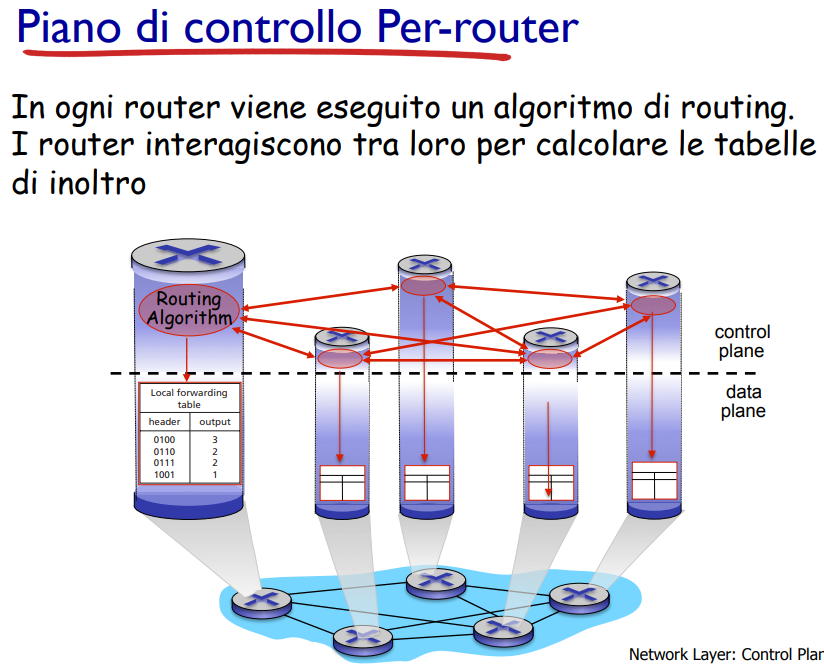
\includegraphics[width=\textwidth]{./img/perrouter.png}
\end{minipage}\hfill
\begin{minipage}{0.48\textwidth}
    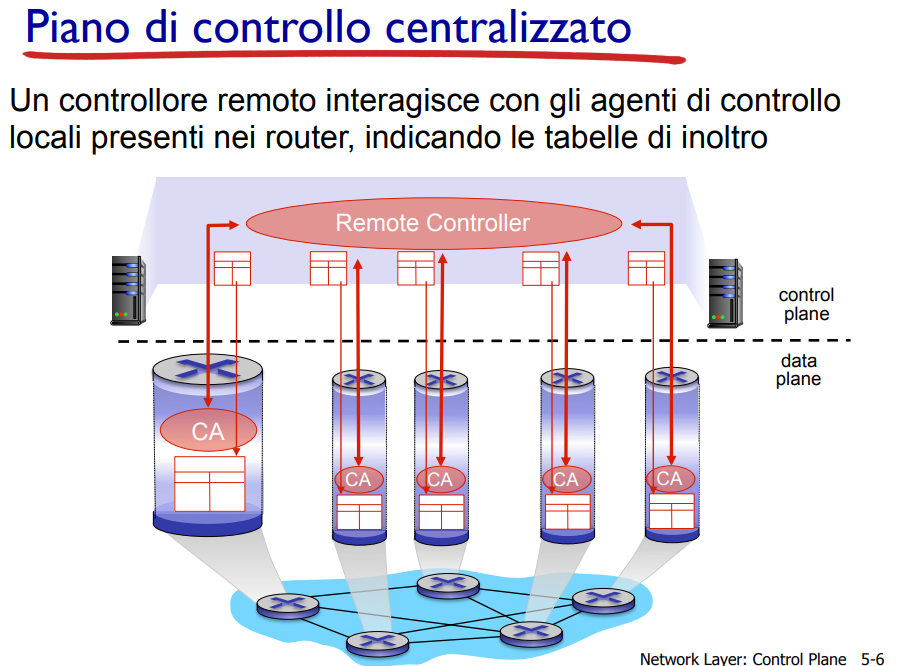
\includegraphics[width=\textwidth]{./img/centralizzato.png}
\end{minipage}
\end{center}

Come mostrato nelle immagini, il controllo per router prevede che ogni router esegua un algoritmo di instradamento e comunichi con gli altri router, mentre il controllo centralizzato prevede un controller remoto che interagisce con gli agenti di controllo locali nei router.

\subsection{Algoritmi di instradamento}
Gli algoritmi di instradamento (routing algorithm) determinano i percorsi a costo minimo tra sorgenti e destinazioni attraverso la rete di router.

\subsubsection*{Grafo di una rete di calcolatori}
Un grafo \(G = (N, E)\) è un insieme \(N\) di nodi (router) e un insieme \(E\) di archi (collegamenti) tra i nodi. Ad ogni arco è associato un costo \(c(x,y)\). Il costo di un percorso è la somma dei costi degli archi lungo il percorso. L'obiettivo è trovare il percorso a costo minimo tra due nodi.

\begin{center}
  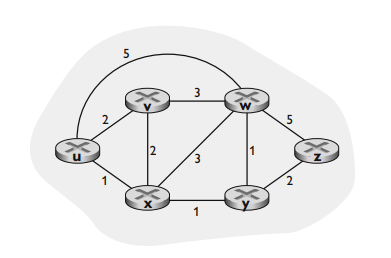
\includegraphics[width=0.7\textwidth]{./img/grafo.png}
\end{center}

\subsubsection*{Definizioni dei grafi}

\begin{itemize}
  \item nodo \textbf{vicino} o \textbf{adiacente}: un nodo y è vicino a un nodo x se (x, y) è un nodo di E. 
  \item \textbf{percorso}: sequenza di nodi (x\_1, x\_2, \dots, x\_p) tali che ciascuna delle coppie (x\_1, x\_2), (x\_2. x\_3), \dots (x\_{p-1}, x\_p) sia un arco di E.
  \item \textbf{percorso a costo minimo} (\textit{least-cost path}): Tra tutti i possibili percorsi tra due nodi, il percorso a costo minimo è quello con il costo totale più basso. 
  \item \textbf{Percorso Più Breve:} Se tutti gli archi del grafo hanno lo stesso costo, il percorso a costo minimo corrisponde al percorso più breve, ovvero quello con il minor numero di collegamenti. 
\end{itemize}

\subsubsection*{Classificazione degli algoritmi di instradamento}
Gli algoritmi di instradamento determinano il cammino a costo minimo e possono essere classificati in base a diversi criteri:
\begin{itemize}
    \item \textbf{Globale o Decentralizzato:}
        \begin{itemize}
            \item \textit{Globale (Link-State):} calcola il percorso a costo minimo tra una sorgente e una destinazione avendo una conoscenza globale e completa della rete. L'algoritmo riceve in ingresso tutti i collegamenti tra i nodi e i loro costi. Questi algoritmi sono spesso utilizzati in reti di piccole e medie dimensioni, dove la conoscenza globale della topologia è fattibile. Un esempio è l'algoritmo di Dijkstra.
            \item \textit{Decentralizzato (Distance-Vector):} il percorso a costo minimo viene calcolato in modo distribuito e iterativo. Ogni nodo elabora un vettore di stima dei costi verso tutti gli altri nodi nella rete. Il percorso a costo minimo viene calcolato in modo distribuito e iterativo, con i nodi che scambiano informazioni con i loro vicini. Un esempio è l'algoritmo di Bellman-Ford.
        \end{itemize}
    \item \textbf{Statico o Dinamico:}
        \begin{itemize}
            \item \textit{Statico:} I percorsi cambiano raramente, spesso a seguito di un intervento manuale. Sono semplici da implementare ma non si adattano ai cambiamenti della rete.
            \item \textit{Dinamico:} I percorsi cambiano al variare del volume di traffico o della topologia della rete. Sono più complessi da implementare ma si adattano meglio ai cambiamenti della rete.
        \end{itemize}
\end{itemize}
